%%%%%%%%%%%%%%%%%%%%%%%%%%%%%%%%%%%%%%%%%%%%%%%%%%%%%%%%%%%%%%%%%%%%%%%%%%%%%%%%
%2345678901234567890123456789012345678901234567890123456789012345678901234567890
%        1         2         3         4         5         6         7         8

%\documentclass[letterpaper, 10 pt, conference]{ieeeconf}  % Comment this line out
                                                          % if you need a4paper
\documentclass[a4paper, 10pt, conference]{ieeeconf}      % Use this line for a4
                                                       % paper
\usepackage{caption, graphicx, amsmath, tabularx, indentfirst, lastpage}    
\usepackage{fancyhdr}
\pagestyle{fancy}
\fancyhf{}
\renewcommand{\headrulewidth}{0.4pt}
\renewcommand{\footrulewidth}{0.4pt}
\cfoot{\thepage\ of 5}                                          
                                                          

\IEEEoverridecommandlockouts                              % This command is only
                                                          % needed if you want to
                                                          % use the \thanks command
\overrideIEEEmargins
% See the \addtolength command later in the file to balance the column lengths
% on the last page of the document



% The following packages can be found on http:\\www.ctan.org
%\usepackage{graphics} % for pdf, bitmapped graphics files
%\usepackage{epsfig} % for postscript graphics files
%\usepackage{mathptmx} % assumes new font selection scheme installed
%\usepackage{times} % assumes new font selection scheme installed
%\usepackage{amsmath} % assumes amsmath package installed
%\usepackage{amssymb}  % assumes amsmath package installed

\title{\Large \bf
Investigating the Relationship between \\ Drugs and Criminal Behaviors / Emotional Stress \\ using Propensity Score Matching, an Observational Study
}

%\author{ \parbox{3 in}{\centering Huibert Kwakernaak*
%         \thanks{*Use the $\backslash$thanks command to put information here}\\
%         Faculty of Electrical Engineering, Mathematics and Computer Science\\
%         University of Twente\\
%         7500 AE Enschede, The Netherlands\\
%         {\tt\small h.kwakernaak@autsubmit.com}}
%         \hspace*{ 0.5 in}
%         \parbox{3 in}{ \centering Pradeep Misra**
%         \thanks{**The footnote marks may be inserted manually}\\
%        Department of Electrical Engineering \\
%         Wright State University\\
%         Dayton, OH 45435, USA\\
%         {\tt\small pmisra@cs.wright.edu}}
%}

\author{Darshan Patel}


\begin{document}



\maketitle
\thispagestyle{fancy}
%\thispagestyle{empty}
%\pagestyle{empty}


%%%%%%%%%%%%%%%%%%%%%%%%%%%%%%%%%%%%%%%%%%%%%%%%%%%%%%%%%%%%%%%%%%%%%%%%%%%%%%%%
\begin{abstract}

To understand the association between smoking cigarette and marijuana and criminal behaviors and emotional stress indicators. The criminal acts studied here are theft, arson and burglary. Signs of emotional stress that were studied include nervousness, hopelessness and worthlessness. 

\end{abstract}


%%%%%%%%%%%%%%%%%%%%%%%%%%%%%%%%%%%%%%%%%%%%%%%%%%%%%%%%%%%%%%%%%%%%%%%%%%%%%%%%
\section{INTRODUCTION}

The use of drugs is a public health problem all over the world. This is of interest for two reasons. One is, the rise of criminal behaviors when indulging in drugs. whereas the other is the indication of mental stress. 

Common crimes that get committed include motor vehicle theft, burglary, arson, DUI, sexual offense, fraud and other violent offenses. There are several factors that can indicate why people undergo these criminal behaviors. From having relationship issues, to financial problems, or feeling of insecurity, people over time have committed crimes to get what they want. An underlying reasoning can also be whether they were in the influence of drugs. For instance, DUI is abbreviation for driving under influence; one can only get committed for this when definitely under the influence of alcohol and drugs. But a more subtle relationship can be dug for other crimes. 

Apart from committing crimes, people often take drugs when they were not feeling good mentally. When one is feeling down due to family problems, school pressure or financial issues, they look to drugs to take away the stress for a temporary amount of time. For instance, in high school, many students enjoy smoking marijuana during school hours to relieve themselves. Signs of mental stress include anxiety, isolation, moodiness, unhappiness and more. 

In this paper, several criminal offenses and mental stress indicators will be studied. The crimes that are looked at theft, arson and burglary. Emotional stress indicators that are looked at are feelings of nervousness, hopelessness and worthlessness. An observational study will be done comparing the use of cigarette and marijuana in 2010 and 2015 to see if there are changes in indications in crime and stress. 


\section{Data}

The data provided for this study will come from the National Survey of Drug Use and Health, done in 2010 and 2015. In these studies, the purpose of the survey was to measure the prevalence of drugs in the United State and find relevant information about users and non-users. The target subject for the survey is the civilian, non-institutionalized population of the United States, who are older than 12 years at the time of the survey. The survey was done using CAI methods as well as holding minimum sample sizes per state. Demographic subgroup estimates were also made due to the large sample sizes. In 2010, $57, 313$ subjects were interviewed whereas in 2015, $57,146$ subjects were interviewed. This is nearly the same number of people in both studies. Furthermore, drugs focused on include tobacco, marijuana, crack, cocaine, hallucinogens, heroin, inhalants, methamphetamine, pain relievers, tranquilizers, stimulants and sedatives. Various information about each drug were collected, such as whether the subject has ever taken them and if so, what age did they first try it, time since they last did it, the frequency of use in the past week, month and year, and more. For specialization, information about different strands of drugs were also noted if the drug label was big. For instance, hallucinogens was broken down into LSD, PCP, mescaline and more. Apart from drug usages, information on peoples' social environment, youth experiences, mental health, depression, consumption of alcohol, substance dependence and abuse, criminal acts, and drug treatment was also surveyed. This survey was done so that many variables could be looked at. In 2015, there were $2,666$ measured variables. This is small decrease from the $3,135$ variables that was collected in 2010. 

To aid this study, and optimize computational performance, a handful of variables were extracted from each year. The drugs that was focused on are cigarette, a form of tobacco, and marijuana. Only if a subject has or has not taken the drug in their lifetime was of concern; meaning, there was surety in the drug usage. In Table I and II, the number of smokers and non-smokers is shown. % latex table generated in R 3.4.3 by xtable 1.8-3 package
% Mon Mar 11 21:02:31 2019
\begin{table}[ht]
\centering
\begin{tabular}{rllll}
  \hline
 Group & 2010 & 2015 & Total in Group \\ 
  \hline
 Control & 27157 & 28236 & 55393 \\ 
  Treatment & 30156 & 28910 & 59066 \\ 
  Total in Year  & 57313 & 57146 & 114459 \\ 
   \hline
\end{tabular}
\caption{Usage of Cigarette}
\end{table}
% latex table generated in R 3.4.3 by xtable 1.8-3 package
% Mon Mar 11 21:02:31 2019
\begin{table}[ht]
\centering
\begin{tabular}{rllll}
  \hline
 Group & 2010 & 2015 & Total in Group \\ 
  \hline
Control & 34433 & 32819 & 67252 \\ 
Treatment & 22839 & 24292 & 47131 \\ 
 Total in Year & 57272 & 57111 & 114383 \\ 
   \hline
\end{tabular}
\caption{Usage of Marijuana}
\end{table}
 From here on outwards, the control group is for subjects that don't smoke the drug whereas the treatment group is for subjects that do indulge in the drug. It can be seen that there are more cigarette smokers than non-cigarette smokers. However, there are less marijuana users than non-marijuana users. As for the criminal offenses, three variables were needed, whether a subject has been arrested and booked for theft in the past $12$ months, and likewise for arson and burglary. Lastly, emotional stress indicators that were of interest are feelings of nervousness, hopelessness and worthlessness. To aid this, only the subjects who felt more stressed during a particular month in the past year were looked at, when comparing their stress level during that one month to the past 30 days of the survey. 

Since this is an observational study and propensity score matching will be leveraged, a few covariates, or demographic information will be needed. The demographic information that was used in this study are gender, age, race and employment status. A breakdown of these demographics features for cigarette is shown in Figure 1. $$ 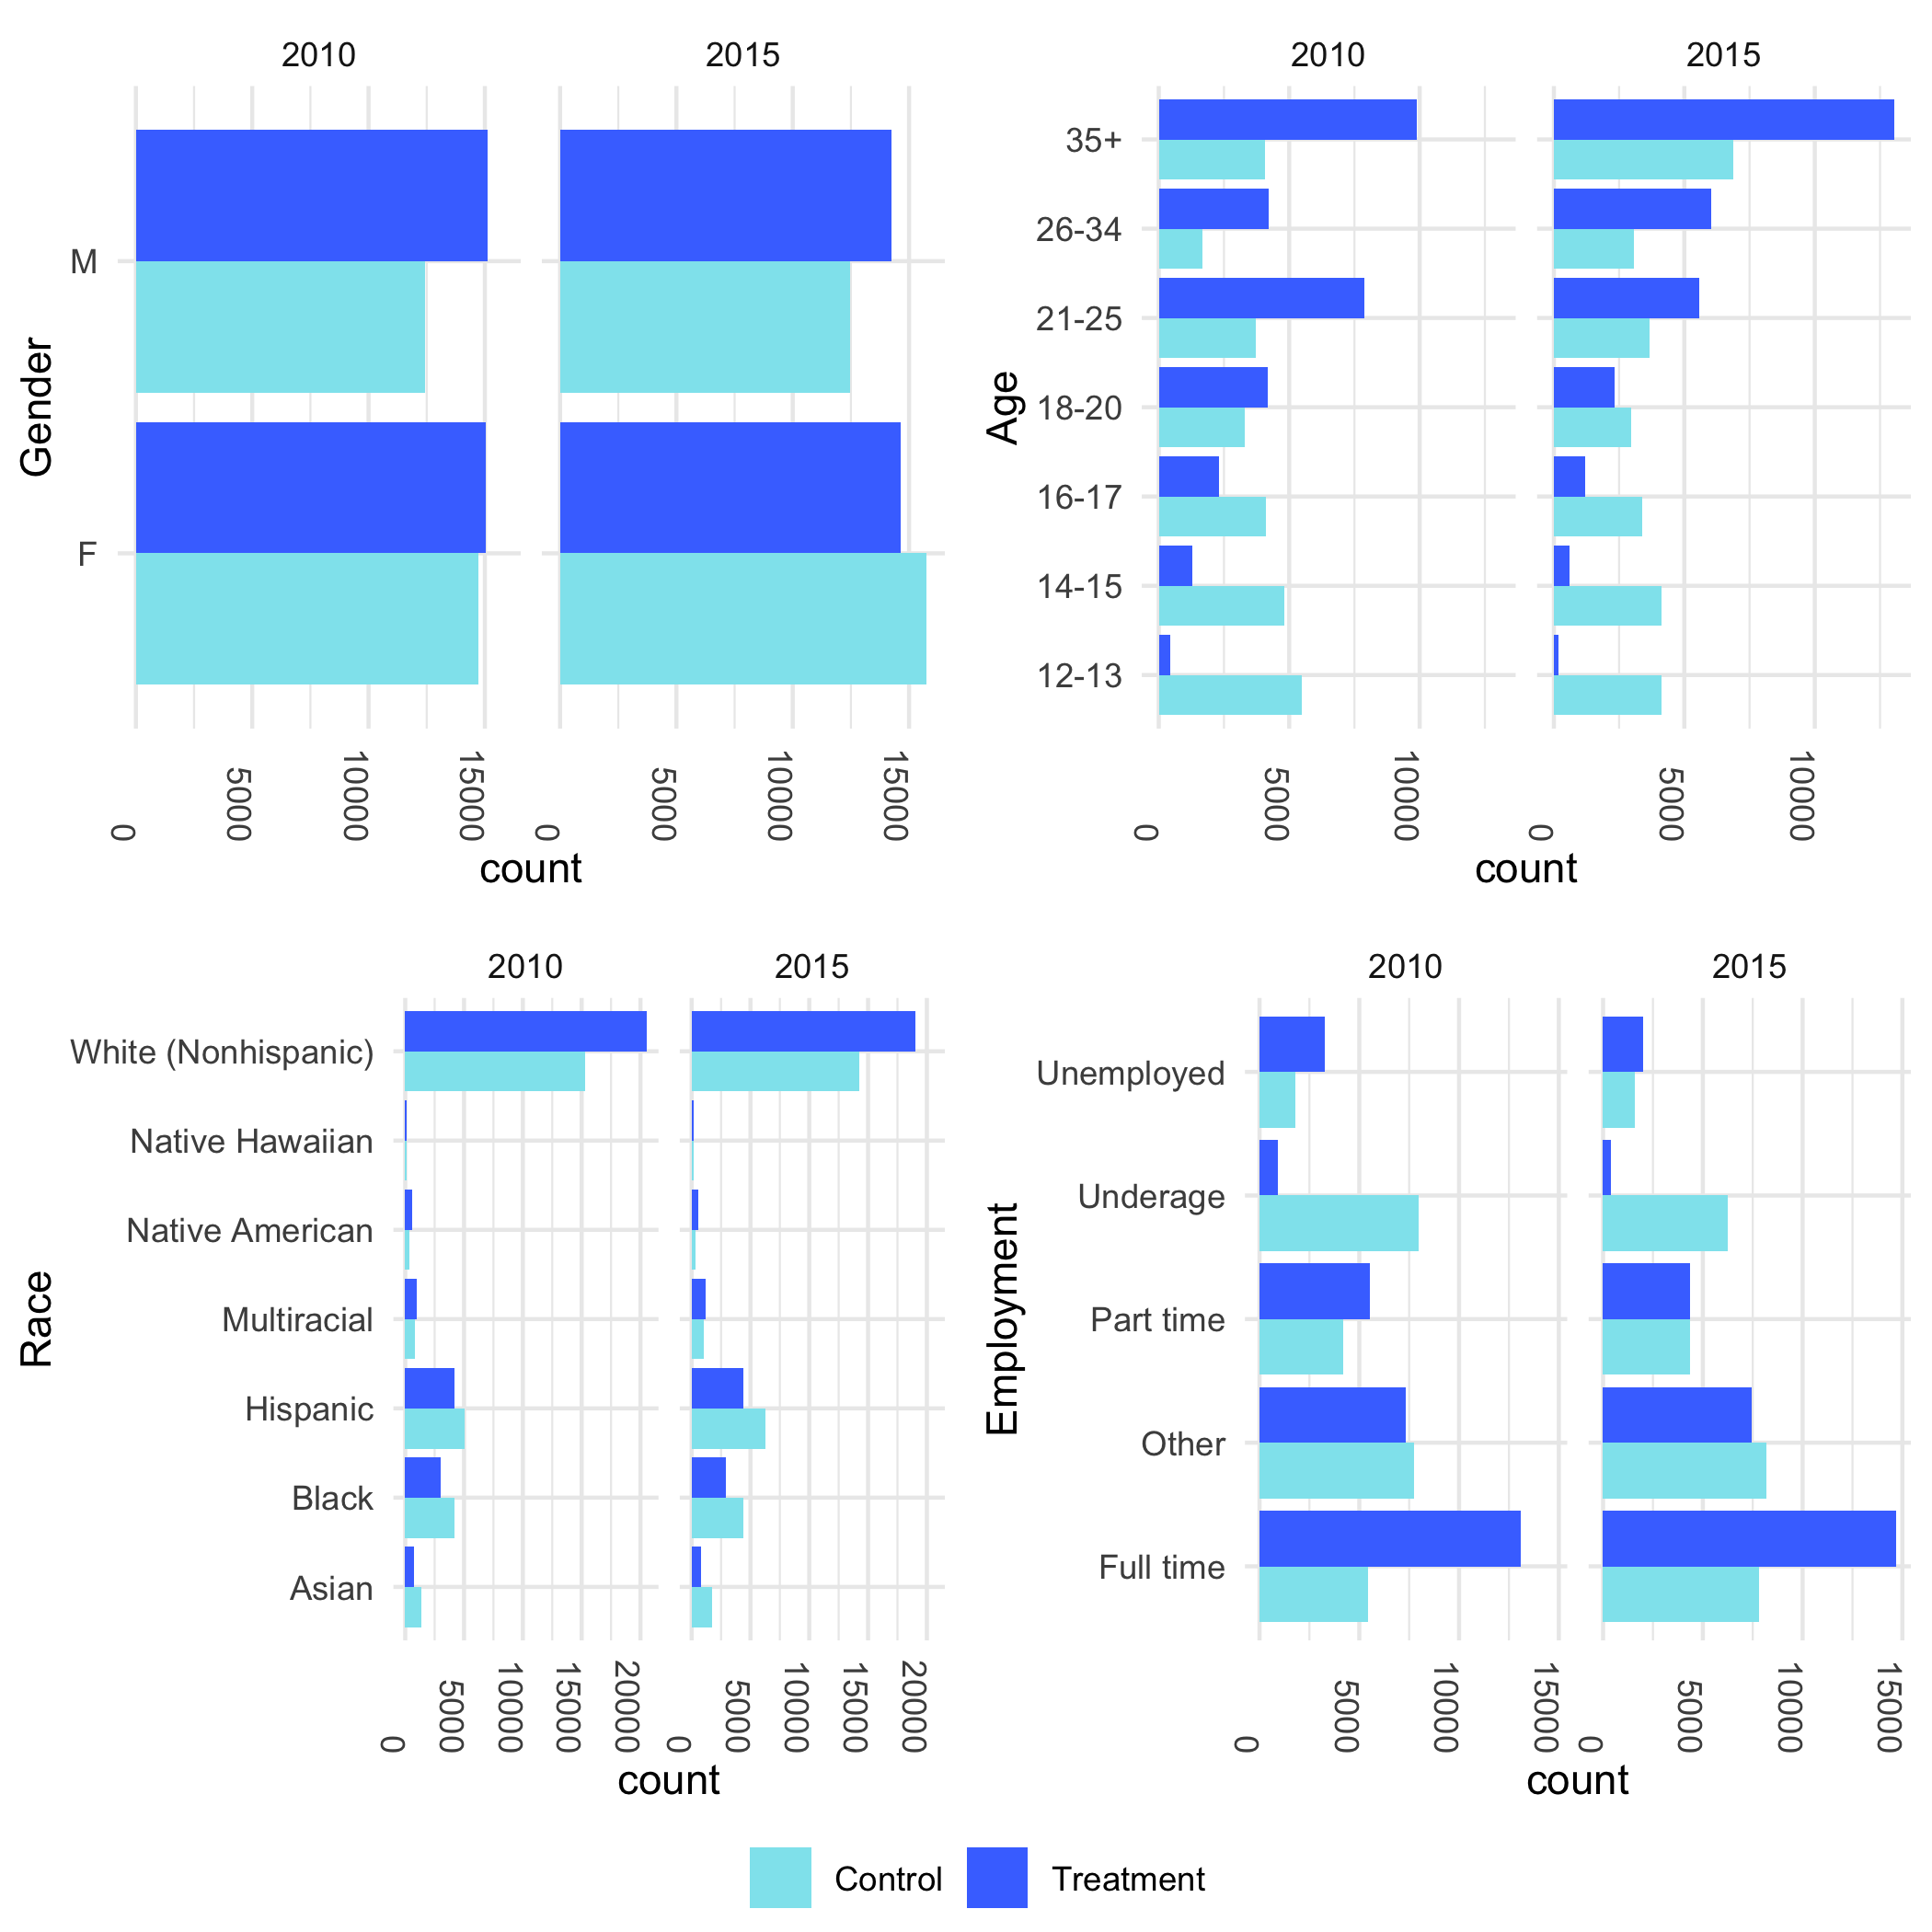
\includegraphics[scale = 0.11]{CigaretteDemographics} $$ \captionof{figure}{Demographic Breakdown of Cigarette \\ } 
\parindent 10pt In this plot, the control group is the subjects who did not smoke cigarette, while the treatment group is the subjects who did. There are several takeaways from this analysis. First, there are more male subjects that have smoked cigarette than those who have not, in both 2010 and 2015. This contrasts with the female subjects; there are more female cigarette smokers than non-smokers in 2010 but not in 2015. In the age distribution, it can be seen that as age increases, there are more smokers generally. In 2010 there is a decrease from the age group of 21-25 years to 26-34 years. Looking at the non-smokers, there does not seem to be any pattern in both 2010 and 2015. When looking at the race demographic, it is apparent that there is a racial imbalance issue in the survey. The white nonhispanic population appear the most in the surveys. Finally, looking at the employment feature, the two highest types are full time employment and ``other" employment. According to the documentation, the ``other" employment refers to people who did not work recently and are not actively looking to be in the labor force. This category could hold people who are not doing anything (in life) or are busy with other commitments. 
$$ 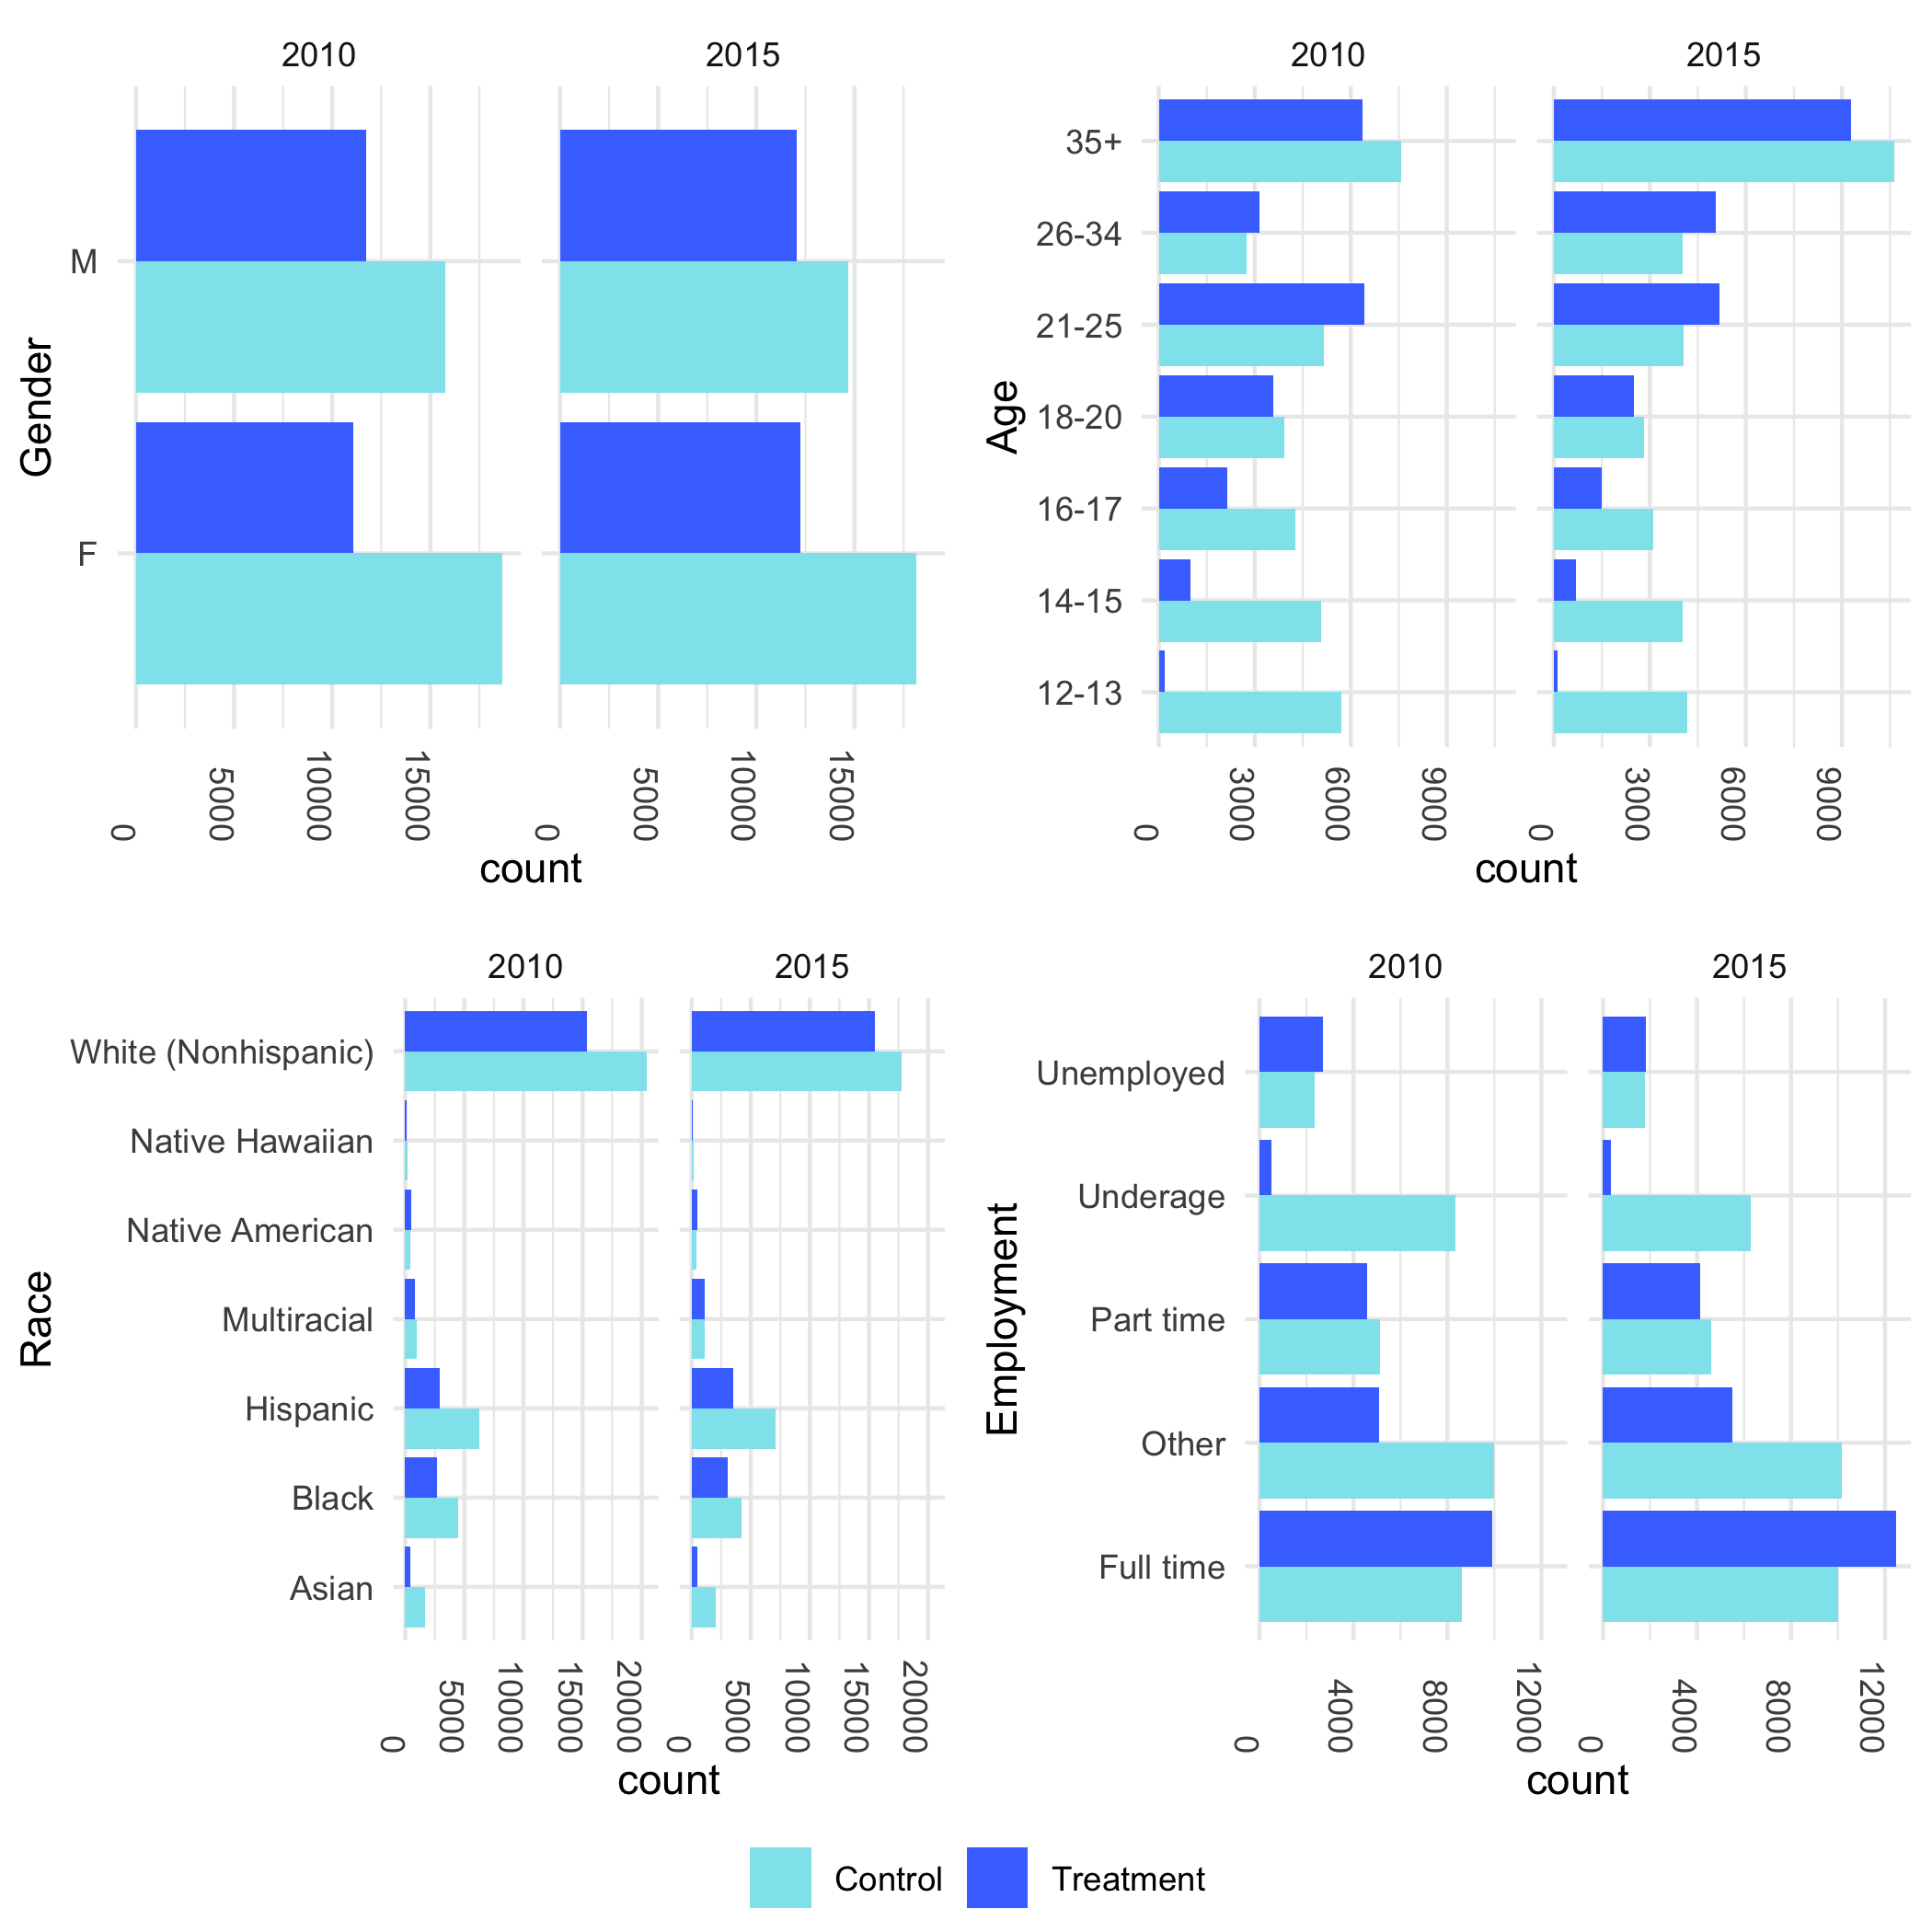
\includegraphics[scale = 0.11]{MarijuanaDemographics} $$ \captionof{figure}{Demographic Breakdown of Marijuana \\ } 
\parindent 10pt A breakdown of the demographics features for marijuana use is shown in Figure 2. Similar analysis as before can be done here. The control group refers to people who have not smoked marijuana whereas the treatment group refers to people who have smoked marijuana. The gender changes are not observed here. There are less marijuana smokers than non-marijuana smokers, with respect to gender, in both 2010 and 2015. In the age plot, it is clear that there are more marijuana smokers as age increases, in both 2010 and 2015. There does seem to be a decrease in smokers in the age range of 26-34 years. Like with the cigarette demographics, there is a huge imbalance in the racial demographics, where white non-hispanics make up most of the population, followed by hispanics and blacks, in both 2010 and 2015. Finally, it is noted that there are many full-time employed subjects in the study for both years.

\section{Methods} 
\parindent 10pt In this observational study, propensity score matching was used to account for the covariates in between the two groups. In all of the analyses, the two groups will be either cigarette/marijuana smokers (treatment group) and non-cigarette/marijuana smokers (control group). With this control/treatment breakdown, a total of $24$ different logistic regression model were made to predict propensity scores. The propensity scores are the probability of using a drug. The explanatory variables used were the covariates and a specific crime/stress variable to study. The covariates were four demographic features of subjects: gender, age, race and employment type. The specific variable to study was one of: theft, arson, sexual offense, nervousness, hopelessness, worthlessness. Thinking in terms of combinations, there are $6$ variables to look at, $2$ different years and $2$ drugs; that makes $24$ different combinations of models that can be made.

After creating the models, for each model, a propensity score distance matrix was built by matching the propensity scores on the data. A caliper was also made on this matrix to only hold distances that had a maximum length of $3$. Using the propensity score distance matrix and the caliper, the propensity scores were matched on the data. The number of matched and unmatched subjects were noted. Using the matched observations, a multiple linear regression model was run to predict the variable at hand, using the covariates and the drug. From the linear model, a coefficient is found for $\beta_{\text{crime}}$ or $\beta_{\text{stress}}$ which assessed the strength of the drug having an impact on the crime or stress indicator. 

\section{Results}
\subsection{Criminal Behaviors}
The propensity score distribution for models with cigarette/non-cigarette smokers and criminal behaviors is shown in Figure 3. $$ 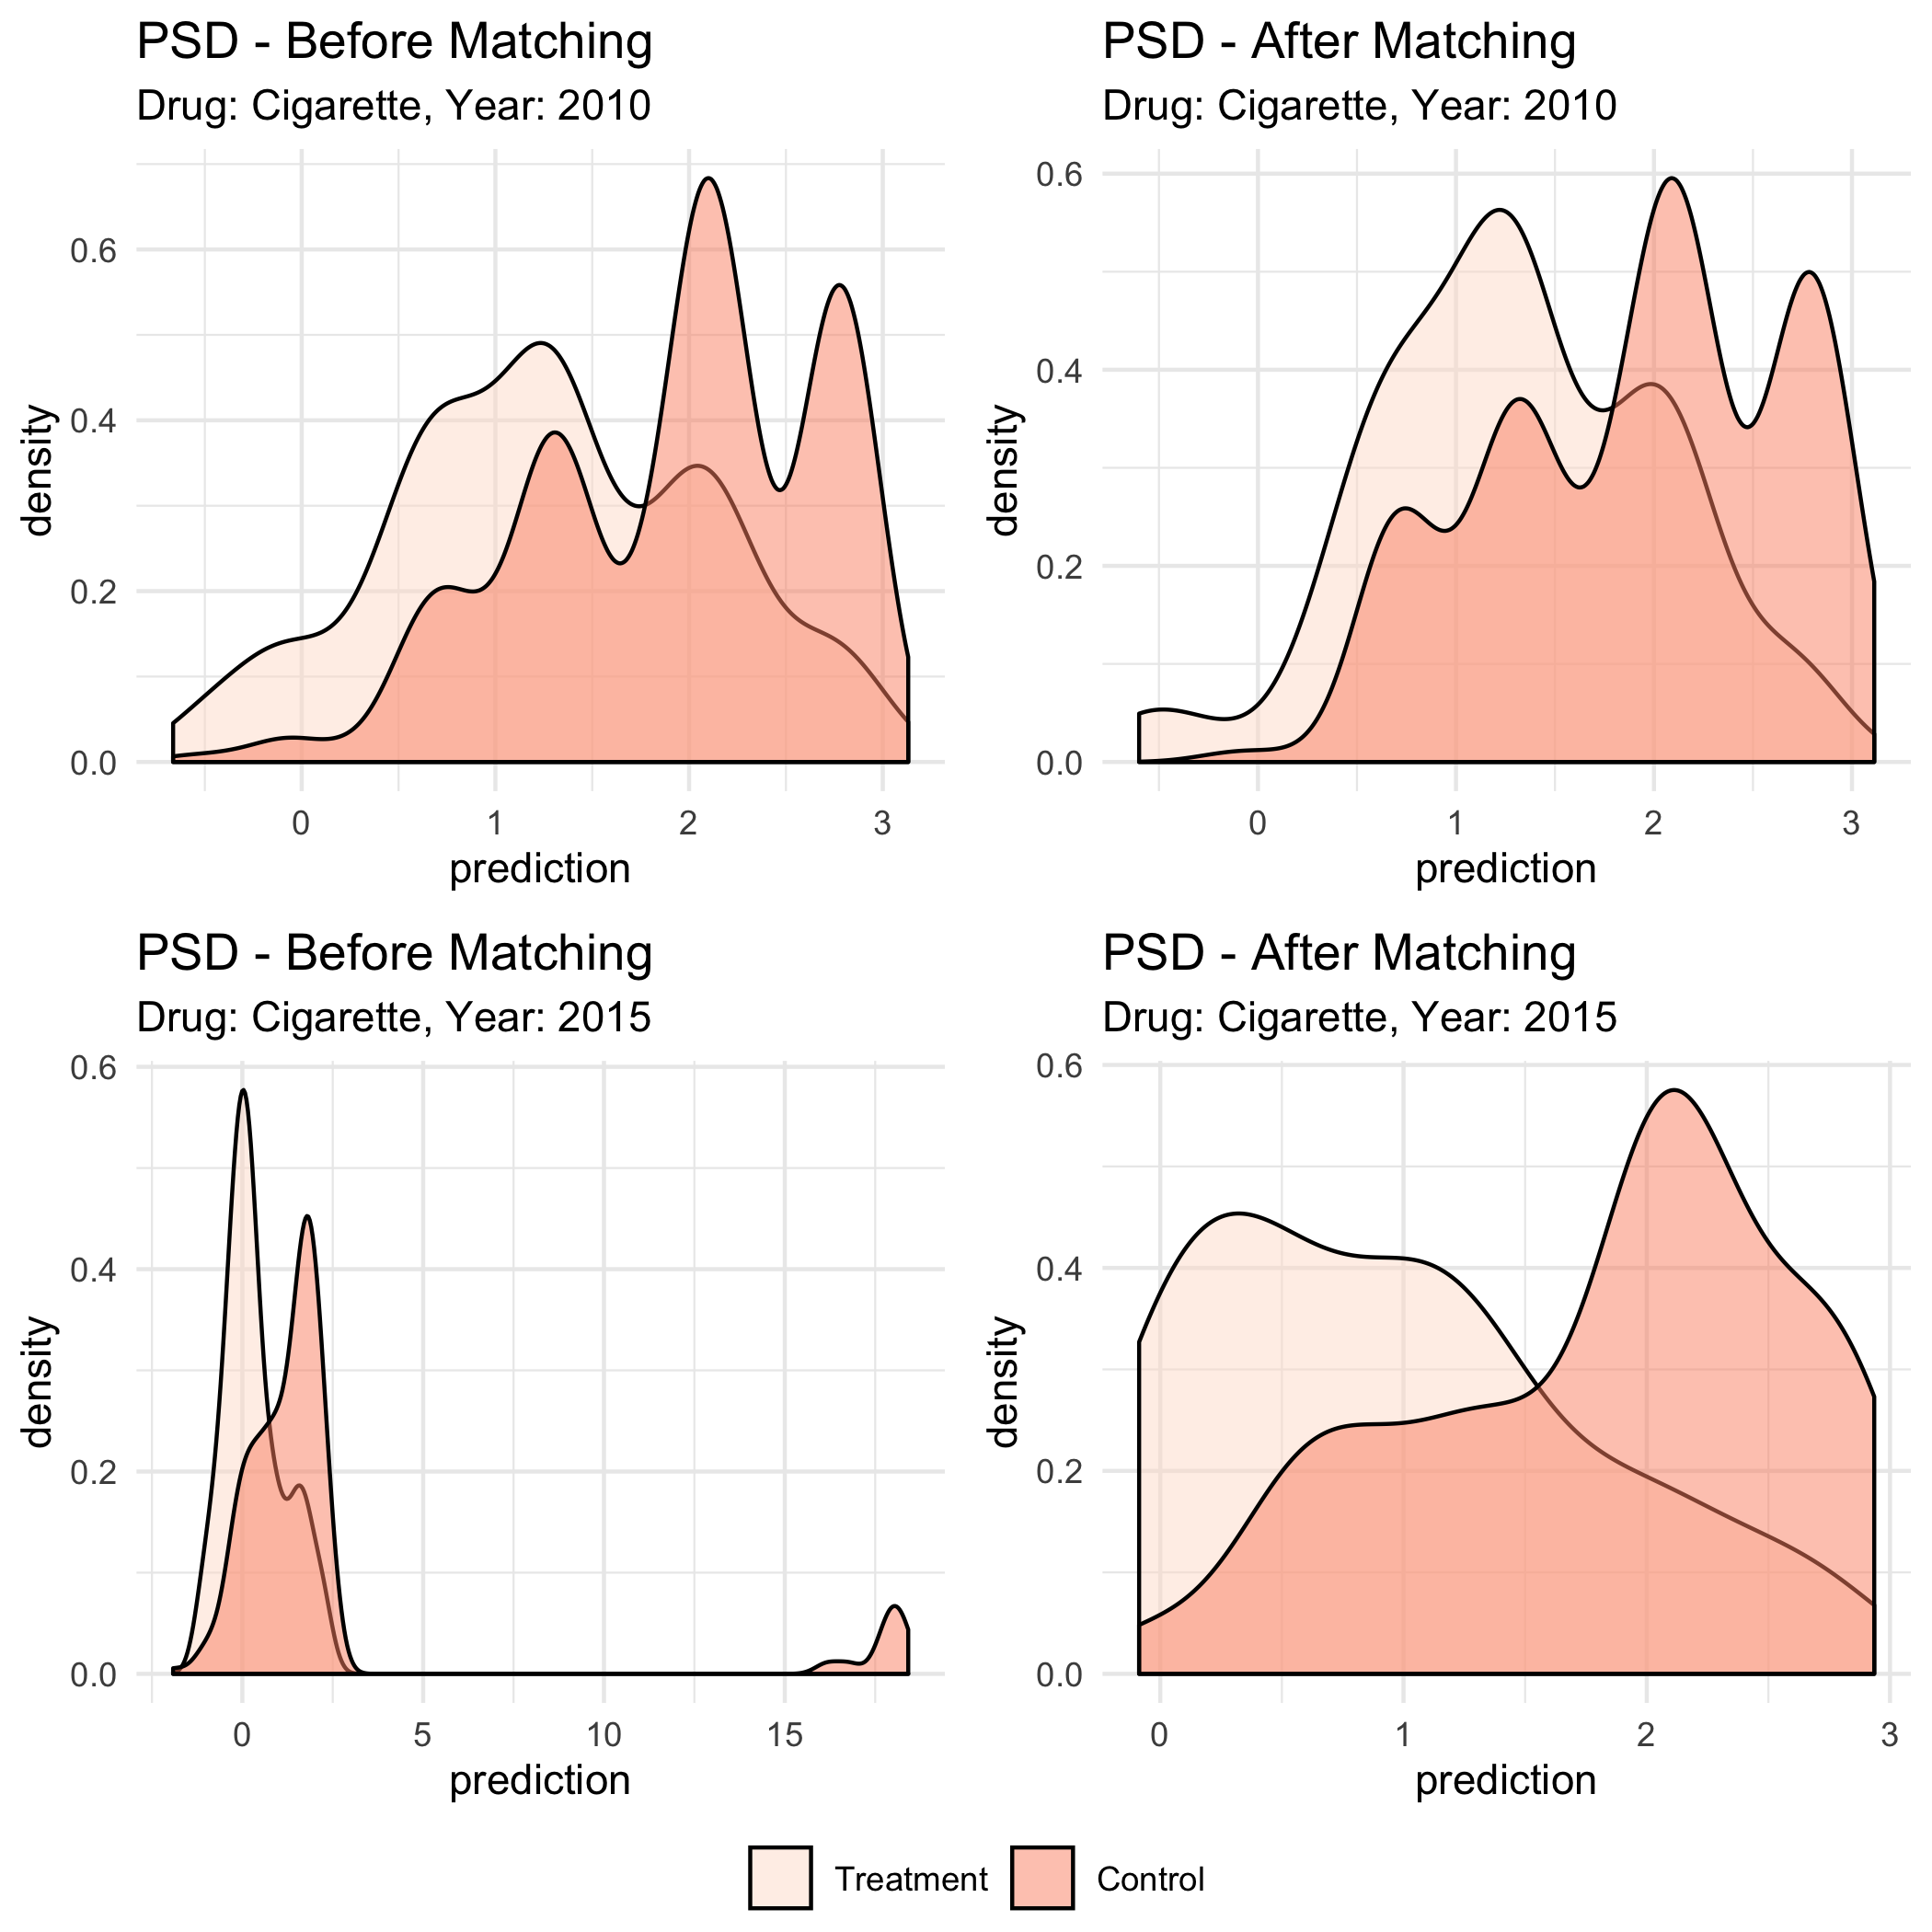
\includegraphics[scale = 0.09]{PSD-Crime-Cig} $$ \captionof{figure}{Propensity Score Density of Cigarette Use and Criminal Behaviors \\ } 
\parindent 10pt By applying propensity score matching, subjects were matched to each other based on their demographic features to balance the ones who did smoke to the ones who didn't smoke using similar demographic features. When doing so, the distribution became flatter and thus more distributed within the range. As for the cigarette smokers in 2015, the extremes on the right hand side got removed by the caliper of width $3$. 

The propensity score distribution for models with marijuana/non-marijuana users and criminal behaviors is shown in Figure 4. The distribution after matching becomes more restricted in terms of its predictions in the case of 2010. In 2015, the range of predictions does not change. What does change though is the removal of predictions on the left hand side from the control group, due to the caliper working to restrict the distances.
$$ 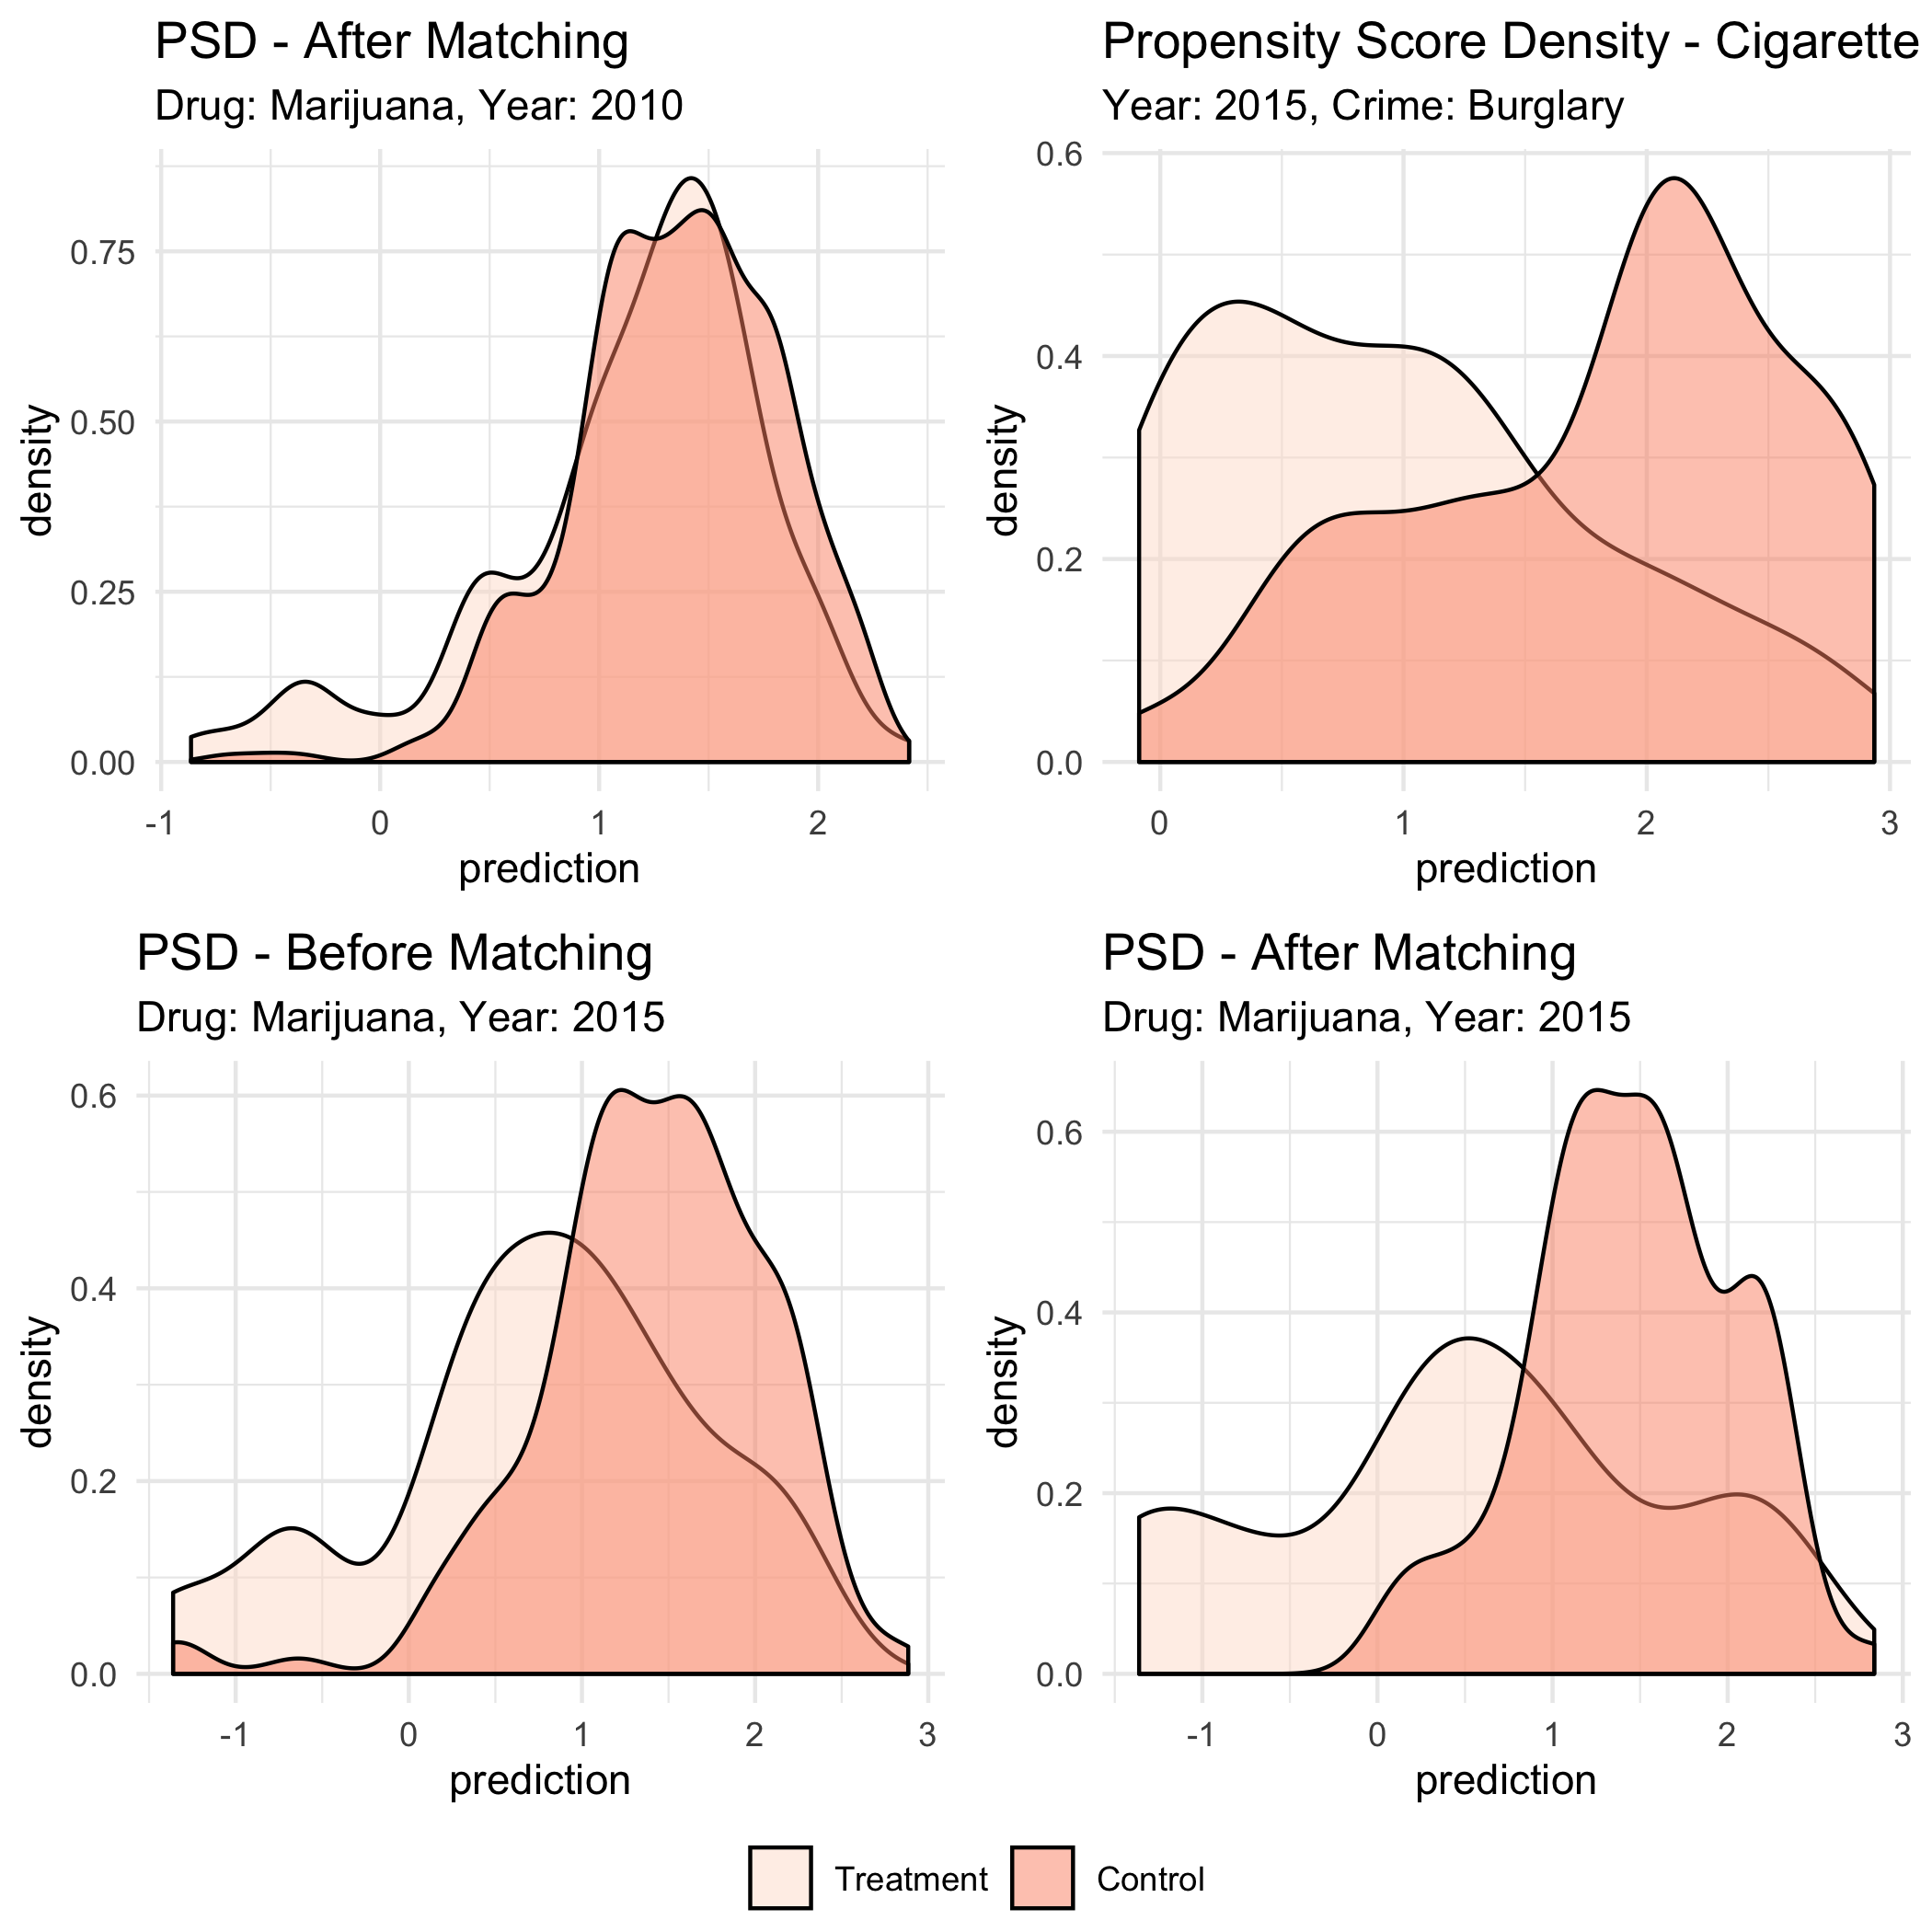
\includegraphics[scale = 0.09]{PSD-Crime-Mar} $$ \captionof{figure}{Propensity Score Density of Marijuana Use and Criminal Behaviors \\ } 

\parindent 10pt The coefficients calculated from running multiple linear regression is shown in Table III.  % latex table generated in R 3.4.3 by xtable 1.8-3 package
% Sun Mar 10 23:30:51 2019
\begin{table}[ht]
\centering
\begin{tabularx}{\columnwidth}{XlXXXX}
  \hline
 & Model & $\beta_{\text{crime}}$ & $n_{\text{m}}$ & $n_{\text{nm}}$ & $p$-value \\ 
  \hline
1 & Cigarette/Theft/2010 & 0.02 & 403 & 1620 & 0.49 \\ 
  2 & Cigarette/Theft/2015 & 0.14 & 109 & 144 & 0.03 \\ \hline
  3 & Cigarette/Arson/2010 & 0.02 & 403 & 1620 & 0.05 \\ 
  4 & Cigarette/Arson/2015 & 0.00 & 109 & 144 &  \\ \hline
  5 & Cigarette/Burglary/2010 & 0.05 & 403 & 1620 & 0.00 \\ 
  6 & Cigarette/Burglary/2015 & $-$0.12 & 109 & 144 & 0.00 \\ \hline
  7 & Marijuana/Theft/2010 & $-$0.02 & 540 & 1345 & 0.51 \\ 
  8 & Marijuana/Theft/2015 & 0.15 &  90 & 182 & 0.04 \\ \hline
  9 & Marijuana/Arson/2010 & 0.01 & 540 & 1345 & 0.12 \\ 
  10 & Marijuana/Arson/2015 & 0.00 &  90 & 182 &  \\ \hline
  11 & Marijuana/Burglary/2010 & 0.04 & 540 & 1345 & 0.00 \\ 
  12 & Marijuana/Burglary/2015 & $-$0.08 &  90 & 182 & 0.05 \\ 
   \hline
\end{tabularx}
\caption{Regression of Crime Variables} 
\end{table}
 It is apparent that only a few coefficients give meaningful insights. At the confidence level of $\alpha  = 0.1$, $4$ of the models gave insignificant coefficient estimates for $\beta_{\text{crime}}$ since its $p$-value was greater than the confidence level. Further modeling technique would need to be done to make them significant. However, a few estimates are significant and those can be evaluated. For instance, for model (2), a model that predicts whether a person will commit an act of theft, based on if they are a cigarette smoker in 2015, the coefficient estimate for $\beta_{\text{crime}}$ is $0.14$. This means that, leaving all covariates (demographic information) constant, if a person does smoke cigarette, then there is an increase of $14\%$ in probability of them committing a theft crime. Whether to say this indicates a strong causal relationship will require further investigation. Nonetheless, since it is not zero, it can be stated that smoking cigarette is associated with theft crimes. Looking back at the same model done in 2010, model (1), $\beta_{\text{crime}}$ is only $0.02$. This is a minuscule value, close to $0$. The $p$-value associated with the model is also high, $0.49$. This states that the coefficient estimate is insignificant. Interpreting it, however, says that when leaving all covariates constant, a smoker has an increase of $2\%$ chance of committing theft compared to a non-smoker. Since the $p$-value is too high, this estimate cannot be trusted, nor can the interpretation have any real meaning. Now, a person who smokes cigarette has an increase of $2\%$ chance of committing arson in 2010 over a non-cigarette smoker, in 2010, when keeping all other variables constant. This is a tiny value. It can be ruled that this happens by chance. The $p$-value associated with the estimate is less than the significant level and so the coefficient estimate is significant. Further investigation would be good. As for the other models in this portion of the study, interesting revelations were made. A non-cigarette smoker in 2015 has an increase of $12\%$ chance of committing burglary over an actual cigarette smoker. This contrasts with the data in 2010 where a smoker has an increase of $5\%$ in probability of committing burglary. Another revelation found is with marijuana smokers and theft. A marijuana smoker has an increase of $15\%$ in probability for committing and being persecuted for theft, over a non-marijuana smoker in 2015, keeping all other demographic information constant. The $p$-value associated with the coefficient estimate is small and so the estimate is deemed reliable. However, when looking at 2010. a non-smoker has an increase in probability of $2\%$ of committing. However this estimate is not reliable. One last revelation that can be made is that in 2015, a non-marijuana smoker is estimated to have an increase in $8\%$ chance of committing burglary over a marijuana smoker, keeping all other variables constant. Other models do not show significant coefficient estimates.
\subsection{Emotional Stress} 
$$ 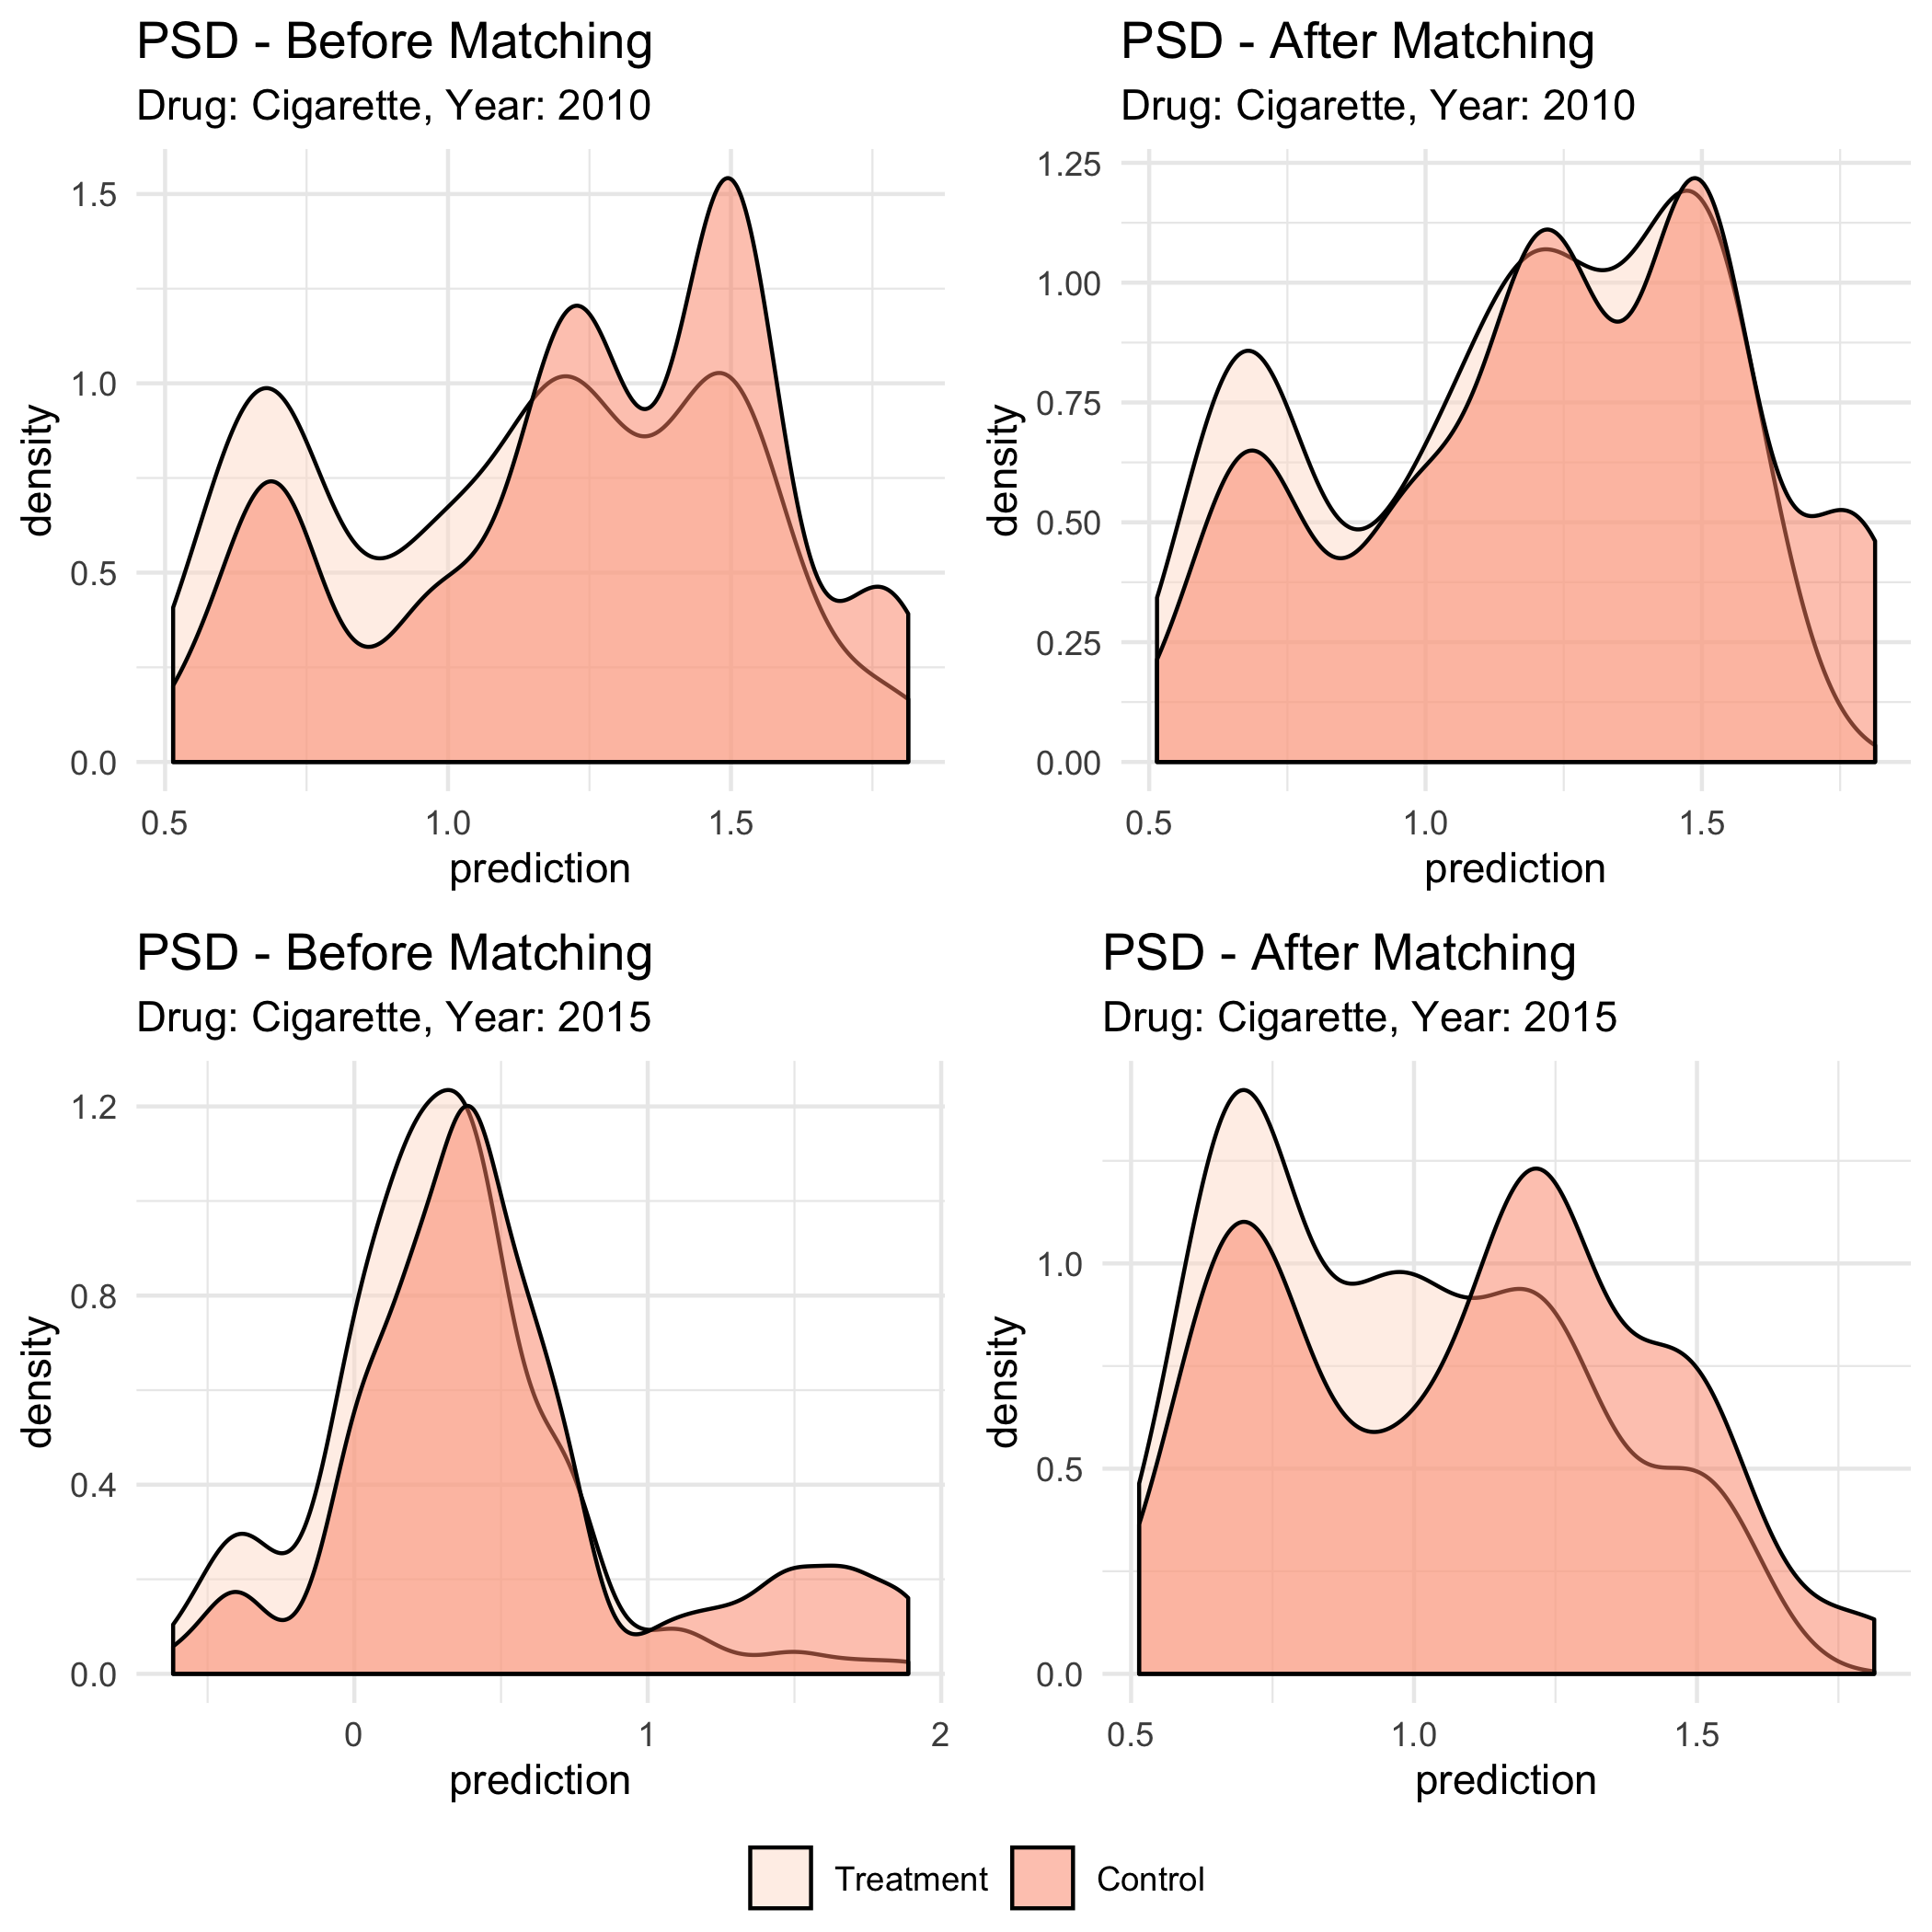
\includegraphics[scale = 0.10]{PSD-MH-Cig} $$ \captionof{figure}{Propensity Score Density of Cigarette Use and Emotional Stress Indicators \\ } 
\parindent 10pt The propensity score distribution for models with cigarette/non-cigarette smokers and emotional stress indicators is shown in Figure 5. 
By leveraging propensity score matching, the distribution of the predictions became alike in 2010 after matching. In the case of 2015, the distribution went from uniform to oddly-shaped. What is noticed, in this case, is that the prediction space is narrower. The control group predictions on the higher end was removed.

The propensity score distribution for models with marijuana/non-marijuana users and emotional stress indicators is shown in Figure 6. Matching did not serve to mane a huge different in either year. The range of the predictions stay relatively the same. In 2015, the predictions for the both groups are less frequent are the higher end. In 2010, the predictions of the treatment group become slightly more uniformly distributed and not left-skewed. The distribution in the year 2015 is bimodal before and after matching.
$$ 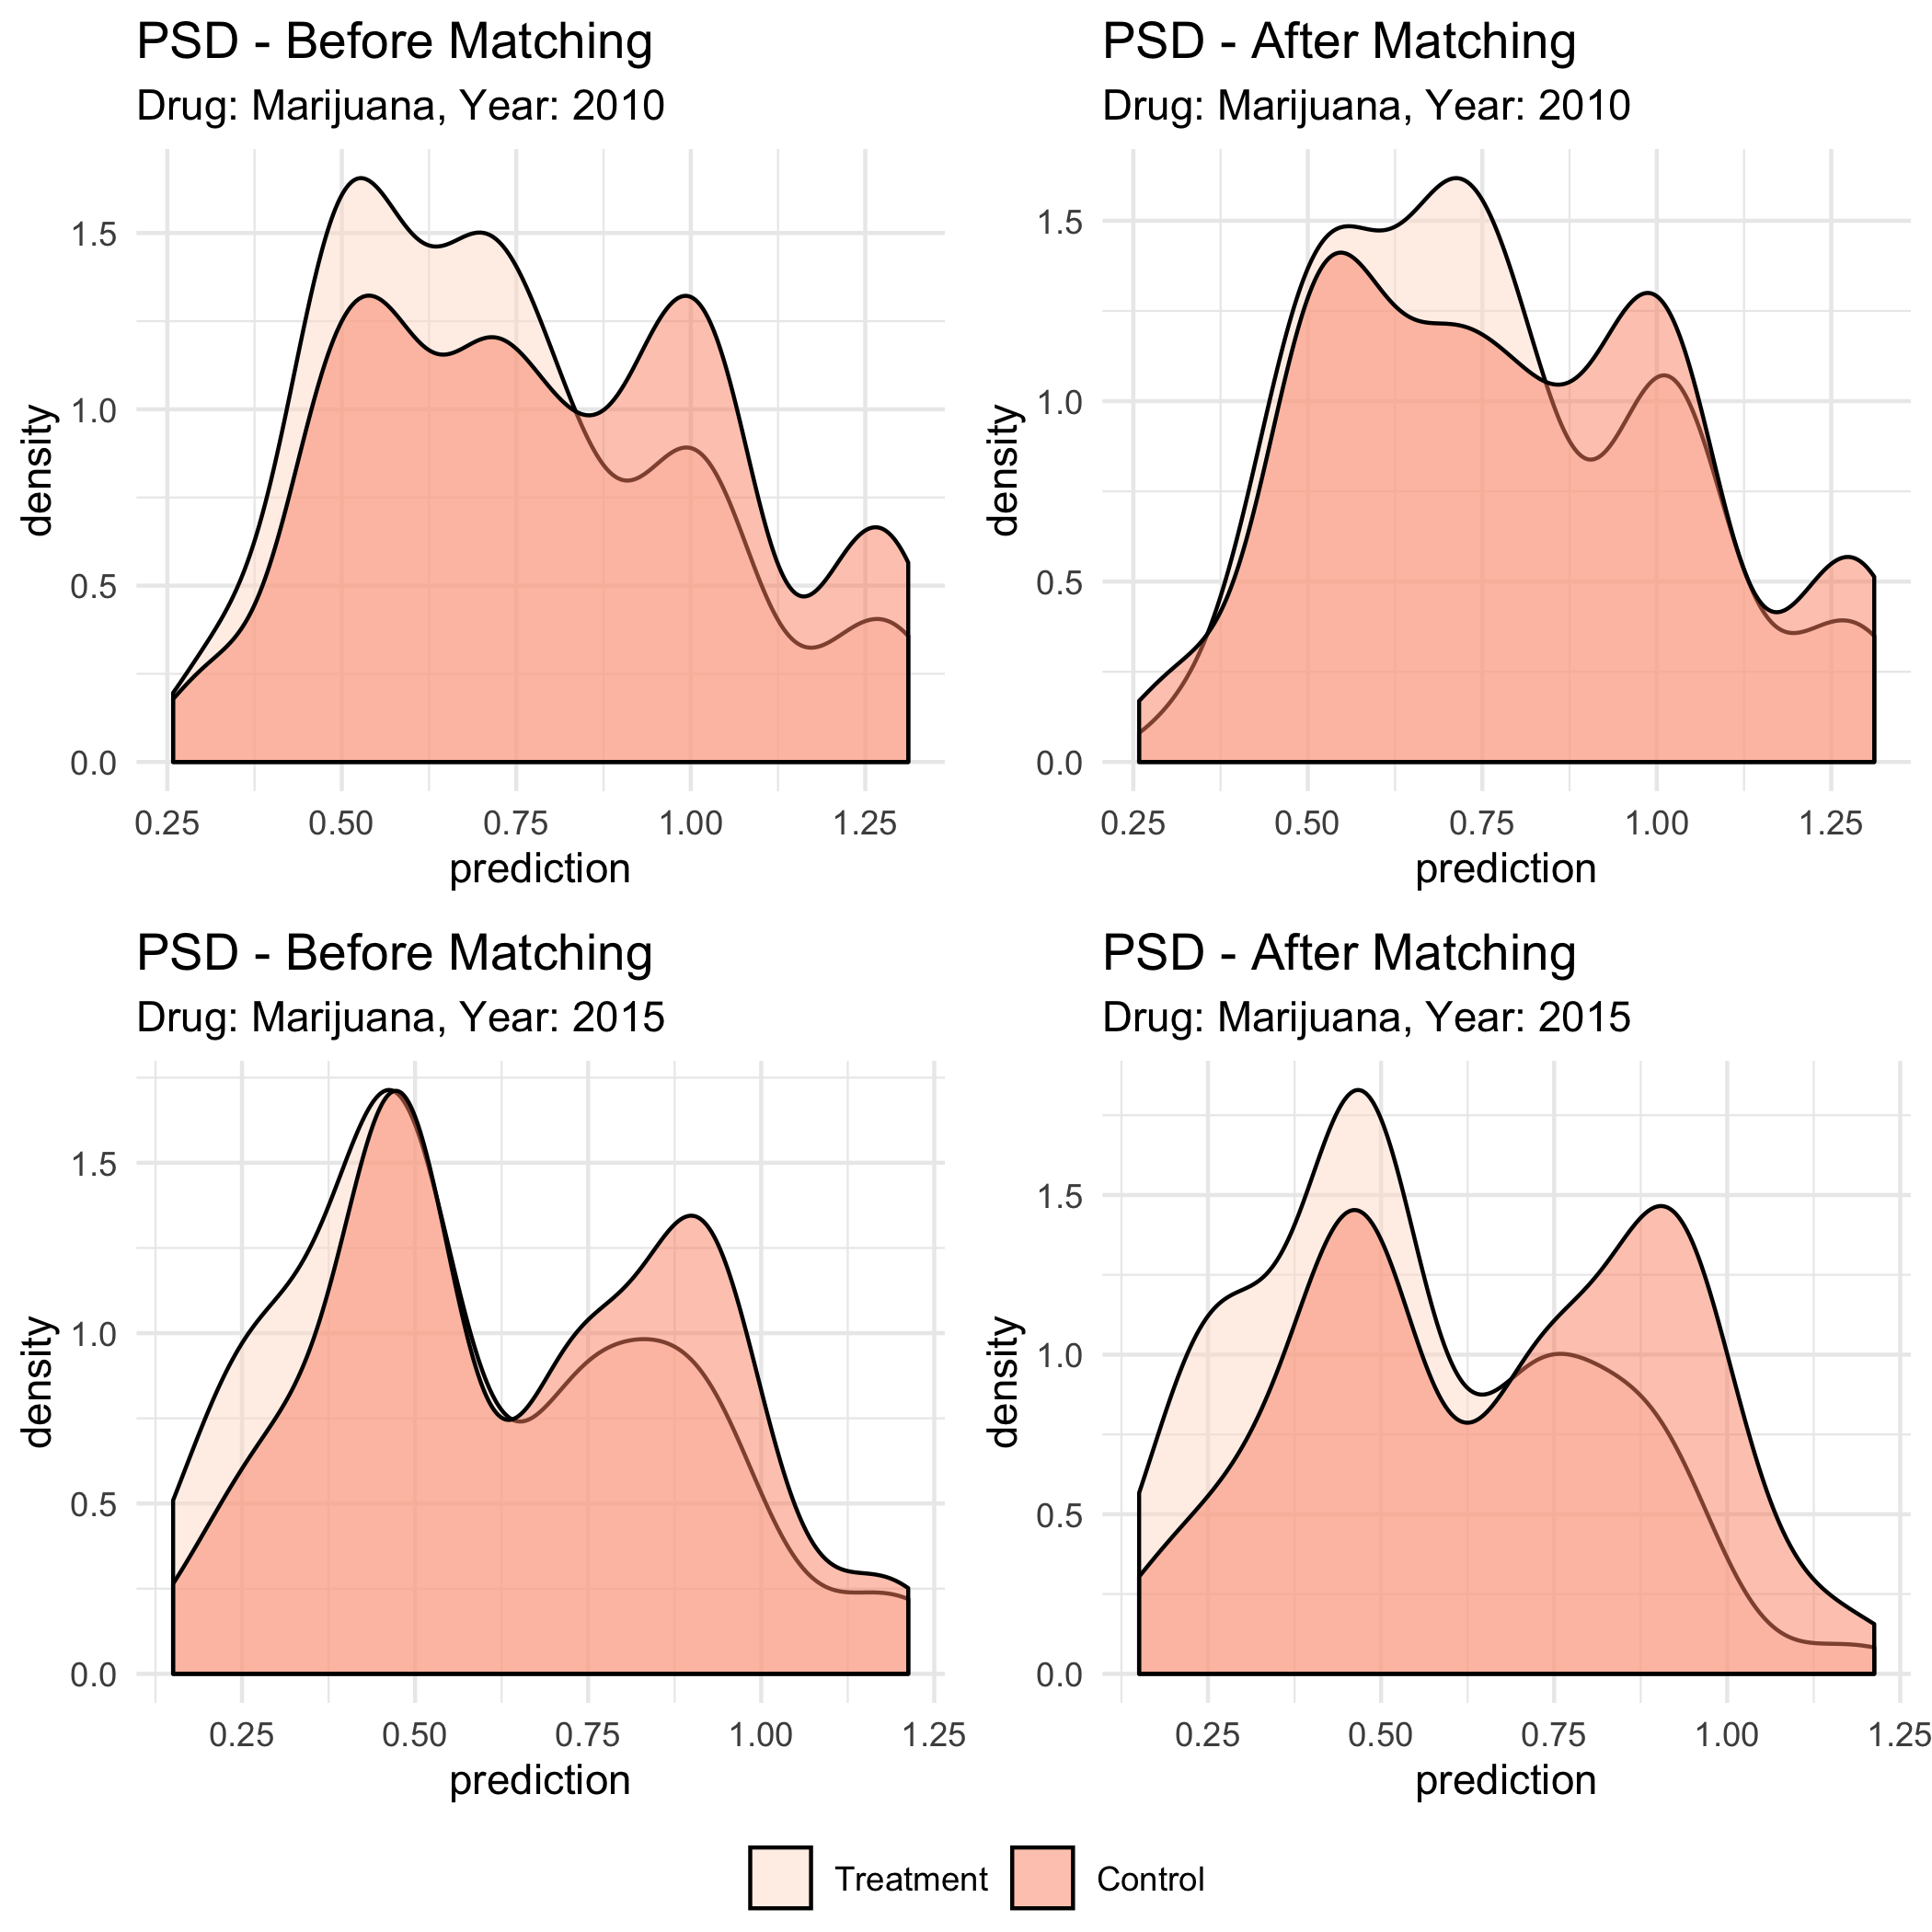
\includegraphics[scale = 0.10]{PSD-MH-Mar} $$ \captionof{figure}{Propensity Score Density of Marijuana Use and Emotional Stress Indicators \\ } 

\parindent 10pt Table IV presents the coefficient estimates found when performing linear regression to predict emotional stress using the covariates and drugs. 
 % latex table generated in R 3.4.3 by xtable 1.8-3 package
% Mon Mar 11 22:54:18 2019
\begin{table}[ht]
\centering
\begin{tabularx}{\columnwidth}{XlXXXX}
  \hline
 & Model & $\beta_{\text{stress}}$ & $n_{\text{matches}}$ & $n_{\text{nm}}$ & $p$-value \\ 
  \hline
1 & Cigarette/Nervousness/2010 & $-$0.03 & 356 & 807 & 0.79 \\ 
  2 & Cigarette/Nervousness/2015 & 0.31 & 185 &  90 & 0.06 \\ 
  3 & Cigarette/Hopelessness/2010 & 0.54 & 356 & 807 & 0.00 \\ 
  4 & Cigarette/Hopelessness/2015 & 0.27 & 185 &  90 & 0.04 \\ 
  5 & Cigarette/Worthlessness/2010 & 0.66 & 356 & 807 & 0.00 \\ 
  6 & Cigarette/Worthlessness/2015 & 0.08 & 185 &  90 & 0.56 \\ 
  7 & Marijuana/Nervousness/2010 & 0.12 & 481 & 557 & 0.21 \\ 
  8 & Marijuana/Nervousness/2015 & $-$0.16 & 161 & 138 & 0.38 \\ 
  9 & Marijuana/Hopelessness/2010 & 0.18 & 481 & 557 & 0.04 \\ 
  10 & Marijuana/Hopelessness/2015 & 0.29 & 161 & 138 & 0.06 \\ 
  11 & Marijuana/Worthlessness/2010 & 0.36 & 481 & 557 & 0.00 \\ 
  12 & Marijuana/Worthlessness/2015 & 0.03 & 161 & 138 & 0.82 \\ 
   \hline
\end{tabularx}
\caption{Regression of Emotional Stress Variables}
\end{table}

Several coefficient estimates are deemed insignificant since the $p$-value associated with estimating the coefficient is greater than the significance level of $\alpha = 0.1$. Nonetheless, a few discoveries can be made. In 2015, a cigarette smoker is predicted to have a $27\%$ increase in probability of having felt hopelessness, when all other covariates are kept constant. This is a huge jump. The $p$-value associated with the estimate is $0.04$ and so the estimate is significant. This is reliable. This is a decrease from the $54\%$ increase in probability in 2010. However, the coefficient estimate has a $p$-value of $0.00$. Whether this estimate can be used requires analysis. Another discovery made is, a marijuana smoker is estimated to have an $18\%$ boost in likeliness to have felt hopelessness in 2010, over non-marijuana smokers, while keeping all other covariates constant. Five years later, this probability jumps to $29\%$. For both of these coefficient estimates, the $p$-value falls below the significance level of $\alpha = 0.1$ and so can be relied on. Coefficient estimates for nervousness can be trusted for cigarette smokers in 2015, where there's a $31\%$ increase in probability of having felt severe nervousness, compared to a non-cigarette smoker, keeping all other variables constant. The coefficient estimates for worthlessness cannot be trusted since the estimations have either very high $p$-values or a $p$-value of $0$.


\section{Conclusion}

In this observational study, an attempt was made to find causal relations between taking certain drugs and criminal behaviors and emotional stress indicators using propensity score matching and regression. In some cases, the matching helped to find subjects that are similar to each other whereas in other, it did not do anything. After matching, when regressing on the crime or stress indicator, a few of the variables stood out to have significance. In the case of the crime variables, cigarette users were shown to have higher probability of committing theft than non-cigarette smokers in one year but not the other. It was not just limited to cigarette; even the use of marijuana was related to a higher chance of having committed theft. As for arson and burglary, conclusions could not be made since the coefficient estimates were too insignificant in both 2010 and 2015. In the case of the emotional stress indicators, nervousness was related to cigarette users in 2015 but not 2010. The same could not be said for marijuana users. Marijuana use was correlated with the feeling of hopelessness though; high increasing percentages of feeling hopelessness paints a mental health sign. This contrasts cigarette users and feeling hopelessness where there is a decrease in probability of feeling this emotion over the course of 5 years. The feeling of worthless could not draw viable conclusions after propensity score matching. 

This study could improve by utilizing other forms of regression could be sought after, such as doubly robust regression or logistic regression itself. In the final step of this study, linear regression models were made to predict a binary value. By using a logistic regression approach with propensity score matching, a more revealing result could be found about the causal relationships. In addition, propensity score matching did not help for some of the datasets, even when calipers were used. Various other forms of matching could be looked at to achieve better matching to yield interpretable results. The next step in this investigation is finding out if other crimes are more related to smokers, or other drug users. Effects of using hallucinogens and inhalants could be sought after. As for cigarette and marijuana, investigation could be done to find out if these drug users do try to get mental health treatment. Nervousness and hopelessness were found to be prominent with smokers. Do the drug users try to get help? An additional factor that was looked at in this study was the comparison of drug use between a $5$ year range, from 2010 to 2015. For most of the models, insignificant estimates were found which could not be used for analysis. An improvement that may help is to look at consecutive years for differences. These are some of the improvements that can be made to this study and further investigation ideas. 

\section*{Acknowledgment}

I would like to acknowledge Professor Frank Yoon, adjunct associate professor of statistics at Fordham University, for his continual effort to educate and provide feedback to students in his observational studies course, despite a low turnout. 







\end{document}
